\documentclass[tikz,border=4pt]{standalone}
\usepackage{amsmath}
\begin{document}
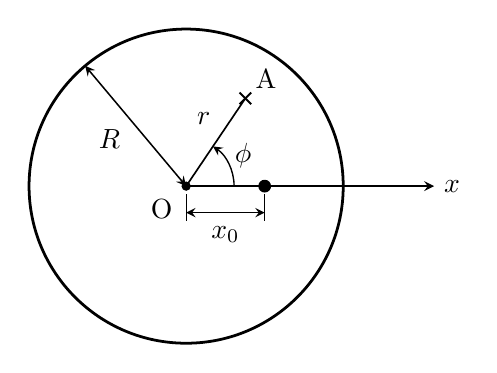
\begin{tikzpicture}[>=stealth, thick, scale=1.05]
  % Hollow conducting cylinder of radius R = 1.9 centered at O(0,0)
  \draw[line width=1.0pt] (0, 0) circle (1.9);

  % x-axis from O to the right
  \draw[->, line width=0.6pt] (0, 0) -- (3.0, 0) node[right] {$x$};

  % Origin O
  \fill (0, 0) circle (1.6pt);
  \node[below left] at (-0.04, -0.04) {$\mathrm{O}$};

  % Radius R arrow (upper left, 130 deg)
  \draw[<->, line width=0.55pt] (0, 0) -- (130:1.9);
  \node[below left] at (130:1.05) {$R$};

  % Off-center wire at (x0, 0) = (0.95, 0)
  \fill (0.95, 0) circle (2.2pt);
  \draw[line width=0.45pt] (0, -0.1) -- (0, -0.42);
  \draw[line width=0.45pt] (0.95, -0.1) -- (0.95, -0.42);
  \draw[<->, line width=0.5pt] (0, -0.32) -- (0.95, -0.32);
  \node[below] at (0.475, -0.36) {$x_0$};

  % Point A at (r, phi) = (1.28, 56 deg)
  \coordinate (A) at (56:1.28);
  \draw[line width=0.6pt] (0, 0) -- (A);
  \draw[line width=0.7pt] (A) ++(-0.07,-0.07) -- ++(0.14,0.14);
  \draw[line width=0.7pt] (A) ++(-0.07,0.07) -- ++(0.14,-0.14);
  \node[above right] at (A) {$\mathrm{A}$};
  \node[above left] at (56:0.75) {$r$};

  % Angle phi
  \draw[->, line width=0.5pt] (0.58, 0) arc[start angle=0, end angle=56, radius=0.58];
  \node at (28:0.78) {$\phi$};
\end{tikzpicture}
\end{document}
